\subsection{Сумма по эквайрингу меньше суммы б/н в Z-отчете}


\begin{itemize}	
	\item Ситуация возникает, когда при проведении платежа, обмен с банком и списание денег с карты клиента не происходит, а чек через фискальный регистратор пробивается. Или при <<лишнем>> отложенном чеке.
	
	

	
	\begin{figure}[H]
		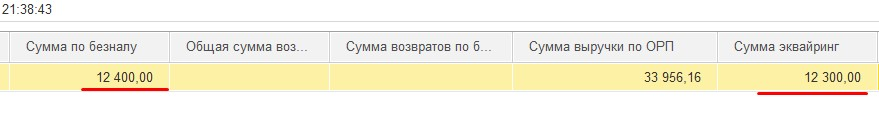
\includegraphics[width=1.0\textwidth]{27.jpg}
		\caption{<<Безнал>>.}
		\label{ris:27.jpg}
	\end{figure}
	Здесь видно, что сумма по безналу на 100 р. больше суммы по эквайрингу.  (Рис.~\ref{ris:27.jpg})
	\item Необходимо создать чек на компьютере товароведа, со следующими особенностями:
	\begin{itemize}[label={--}]
		\item Вид операции <<Возврат>>
		\item Вид оплаты <<Платежная карта>>
		\item На необходимую сумму
		\item Сегодняшним днем
	    \item Используя для этого тот товар, который \textbf{продавался сегодня по этой кассе, по безналу!} 
	\end{itemize}

%	\begin{myquote}

%	\end{myquote}

	\begin{warning}
	\textbf{Внимание!!! Нельзя использовать для чеков коррекции алкоголь!!!}
	\end{warning}
	
	\item Чек записать
	\item Перейти на кассовый компьютер 	
	\item Пробить его согласно «инструкции для кассиров п2.1 параграф <<Г>>
		
    
	
\end{itemize}
